\chapter{Visualization System \label{ch:visualizer}}

It is extremely important to consider the way in which the system presents plots
to the user as that can change the way the user perceives the data. Furthermore,
user interactivity is a critical component of high dimensional analysis as noted
earlier~\cite{lius2016}. (see paragrapah below)

Regardless of whether high dimensional data visualization methods are
computationally heavy or interaction heavy, user interactivity is still a vital
component for processing high dimensions for visualization; it is simply a
question of what degree~\cite{lius2016}. We develop a system that first learns
what visual patterns the data analyst finds promising, querying the user where
the decision tree is ambiguous. It then automatically iterates through thousands
of possible plots. Finally, it suggests relationships to exclude or include,
which it believes to match the data analyst's interests, and their corresponding
plots. This allows users to compare and contrast visual feedback with numerical
algorithms for improved model selection.

User provides numerical graphical model and data that they wish to
analyze/confirm visually $\rightarrow$ program analyzes the plots among edges
that do exist in the graphical model and extract relevant features
(\ref{sec:visualizer:features}) $\rightarrow$ initialize the decision tree given
the resulting data (\ref{sec:visualizer:al:tree}) $\rightarrow$ perform a
line-up test to determine how accurate the initialized tree is $\rightarrow$ 
selectively pick plots corresponding to ambiguous parts of the tree
(\ref{sec:visualizer:al:alplotgeneration}) $\rightarrow$ periodically generate
line-up tests from ambiguous parts of the tree to confirm the current iteration
of the decision tree is ``correct'' (\ref{sec:visualizer:al:lineup})
$\rightarrow$  if the user passes a number of line-up tests, display the final
classifier and heat map (\ref{sec:visualizer:plotgeneration:user}) $\rightarrow$
allow user to tweak if desired $\rightarrow$ output
(\ref{sec:visualizer:plotgeneration:feedback})

\section{Scatterplot characterization}
\label{sec:visualizer:scatterplot}

\subsection{Characteristics of a ``good'' plot}
\label{sec:visualizer:scatterplot:goodplot}

The simplest scatter plot is one without any transformations on the data. This,
however, may not be the best way to ascertain independence for the user. This
notion is illustrated in Figure~\ref{fig:visualizer:cdf}. The left plot appears
to be independent as it's a cluster of points near the origin, but it's not
entirely clear due to the multitude of stray points outside of $y\in (-2,2)$ 
and $x\in(-1.5,1.5)$. By looking at the outliers, it could also be argued that 
there is some dependency. However, applying the CDF in both directions creates 
a plot distributed on (0,1). This transformation is non-destructive and 
preserves dependency in the data if it exists. The data is clearly independent 
as the points appear to be uniformly distributed within the box.

\begin{figure}[htb]
	\begin{center}
		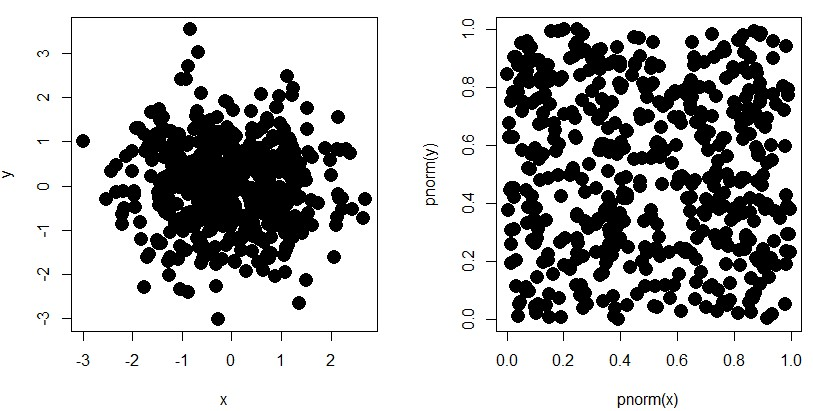
\includegraphics[width=0.75\linewidth]{ch-visualizer/figures/cdf}
		\caption[A plot of $y$ against $x$ after the CDF is applied in both
		directions.]{A plot of $y$ against $x$ with no transformation (left) 
		and after
			the CDF is applied in both directions (right). The code for this 
			example may be
			found in Appendix~\ref{sec:appendicies:cdf}}
		\label{fig:visualizer:cdf}
	\end{center}
\end{figure}

Restricting the scatter plot to a unit box allows analyst's visual systems to 
focus on locations where there is low spatial frequency, which is ideal for 
detecting dependence~\cite{hofert2016}. The effects of this concept can be 
progressively observed from left to right in 
Figure~\ref{fig:visualizer:hofertoldford} below.

\begin{figure}[htb]
	\begin{center}
		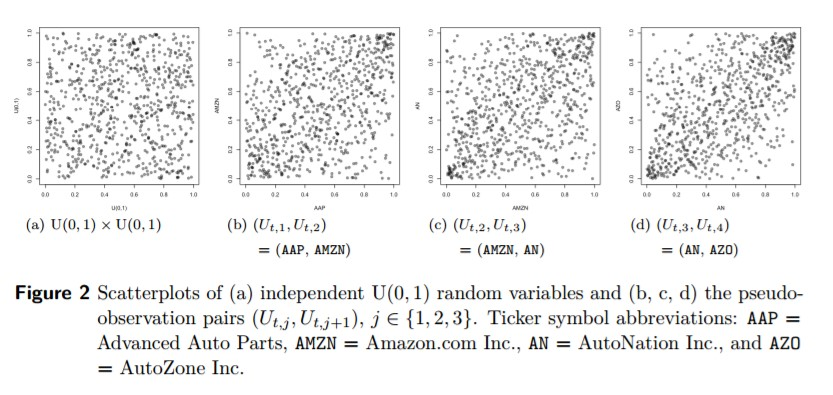
\includegraphics[width=1\linewidth]{ch-visualizer/figures/hofertoldford}
		\caption[Transformed scatter plots of independent $U(0,1)$ random 
		variables and pseudo-observation pairs $(U_{j},U_{j+1}),j\in 
		\{1,2,3\}$ which are more correlated the larger $j$ is.]{\textit{(a):} 
		Transformed scatter plots of independent $U(0,1)$ random variables. 
		\textit{(b,c,d):} Transformed scatter plots of the pseudo-observation 
		pairs $(U_{j},U_{j+1}),j\in \{1,2,3\}$. The variables are clearly more 
		correlated as $j$ increases; this trend can easily be observed due to 
		the nature of the unit box. Ticker abbreviations: 
		AAP = Advanced Auto Parts ($U_1$), AMZN = Amazon.com Inc. ($U_2$), 
		AN = AutoNation Inc. ($U_3$), AZO = AutoZone Inc. ($U_4$).
		Figure from Hofert and Oldford 2016 with slight 
		modifications~\cite{hofert2016}}
		\label{fig:visualizer:hofertoldford}
	\end{center}
\end{figure}

\subsection{Feature extraction from plot}
\label{sec:visualizer:scatterplot:features}

In order for the active learning classifier to properly understand and classify 
all $n \choose 2$ scatter plots in stage 1 and 2
(Sections~\ref{sec:visualizer:al} and~\ref{sec:visualizer:plotgeneration}), 
characteristic features must be extracted from each pairwise scatter plot. The 
more useful criteria there are, the more sophisticated the classification will 
be.

\subsubsection{Numerical features}

Our goal is to quantify various features of a scatter plot for the computer, 
and that does include numerical features. The following features are currently 
implemented in the VS: 

\tablespacing
\begin{itemize}
	\item \textbf{Correlation coefficients and their $p$-values:} Examples 
	include Pearson's, Spearman's, Kendall's, and distance correlation. See 
	Section~\ref{sec:intro:correlation} for more details on the various types 
	of coefficients.
	\item \textbf{Kullback-Leibler divergence criterion:}
	\item \textbf{Chi-square test of independence and its $p$-value:}
\end{itemize}
\bodyspacing 

\subsubsection{Visual features}

What is more challenging is to find a way to quantify the visual features of 
scatter plots. This may be done by looking for concentration of points in 
various spaces of the plot domain. The following features are currently 
implemented in the VS: 

\tablespacing
\begin{itemize}
	\item \textbf{Middle box criterion:} The percentage of points near the 
	center of the plot
	\item \textbf{LR criterion:} The percentage of points that lie above and 
	below the linear regression line
	\item \textbf{Clustering criterion:} The percentage quantile of the ratio 
	between the largest and next-largest distance
	\item \textbf{Visual trend criterion:} This is computed as 
	max(PosTrendCriterion, NegTrendCriterion). The positive trend criterion 
	(PosTrendCriterion) is computed from the percentage of points in the bottom 
	left and upper right while the negative trend criterion (NegTrendCriterion) 
	is computed from the percentage of points in the upper left and 
	bottom right. A higher visual trend criterion value suggests a greater 
	visual trend. 
\end{itemize}
\bodyspacing
\section{Active learning (Stage 1)}
\label{sec:visualizer:al}

The main goal of stage 1 is to learn the user's interests. This requires the 
system to select (``query'') data (which are $n$ characterizations of $d\choose 
2$ plots in the case of the VS as described in 
Section~\ref{sec:visualizer:scatterplot:features}) for the analyst (the 
``oracle'') to label (classify). The learner may then utilize a classification 
model (LDA, QDA, naive bayes, decision tree, random forest, logistic 
regression, etc.) that trains on labeled data to ``learn'' user interests. The 
user's interests are encoded in a classifier (some instance of the 
classification model) that is applied to automatically label the rest of the 
data (For more on the 
semantic differences between ``classification model'' and ``classifier'', see 
Figure~\ref{fig:visualizer:al:tree}). As such, it is important to make the 
process as efficient as possible to avoid redundancy for the end user. There 
are various methods that may be used for querying in stage 
1~\cite{dasgupta2011}:

\tablespacing
\begin{itemize}
	\item \textbf{Supervised learner}: This learner queries a single, random 
	subset of all unlabeled data. It ignores the rest of the data when refining 
	the classifier
	\item \textbf{Semisupervised learner}: Similar to a supervised learner, a 
	semisupervised learner queries a single, random subset of all 
	unlabeled data but proceeds to utilize the remaining unlabeled data to 
	better inform the final classifier
	\item \textbf{Active learner}: An active learner selects its queries in a 
	non-random, intelligent manner to reduce the hypothesis space $\mathcal{H}$ 
	of all possible classifiers that may explain the data.
\end{itemize}
\bodyspacing

It has been 
shown that when a learning algorithm is allowed to choose its next query, it 
performs better with less training; as such, we choose to utilize active 
learning to select the plots to be queried by the oracle in stage 
1~\cite{settles2010}. Chapter~\ref{ch:al} goes into detail on different active 
learning methodologies as this section is primarily focused on its role in the 
system.

\begin{figure}[htb]
	\begin{center}
		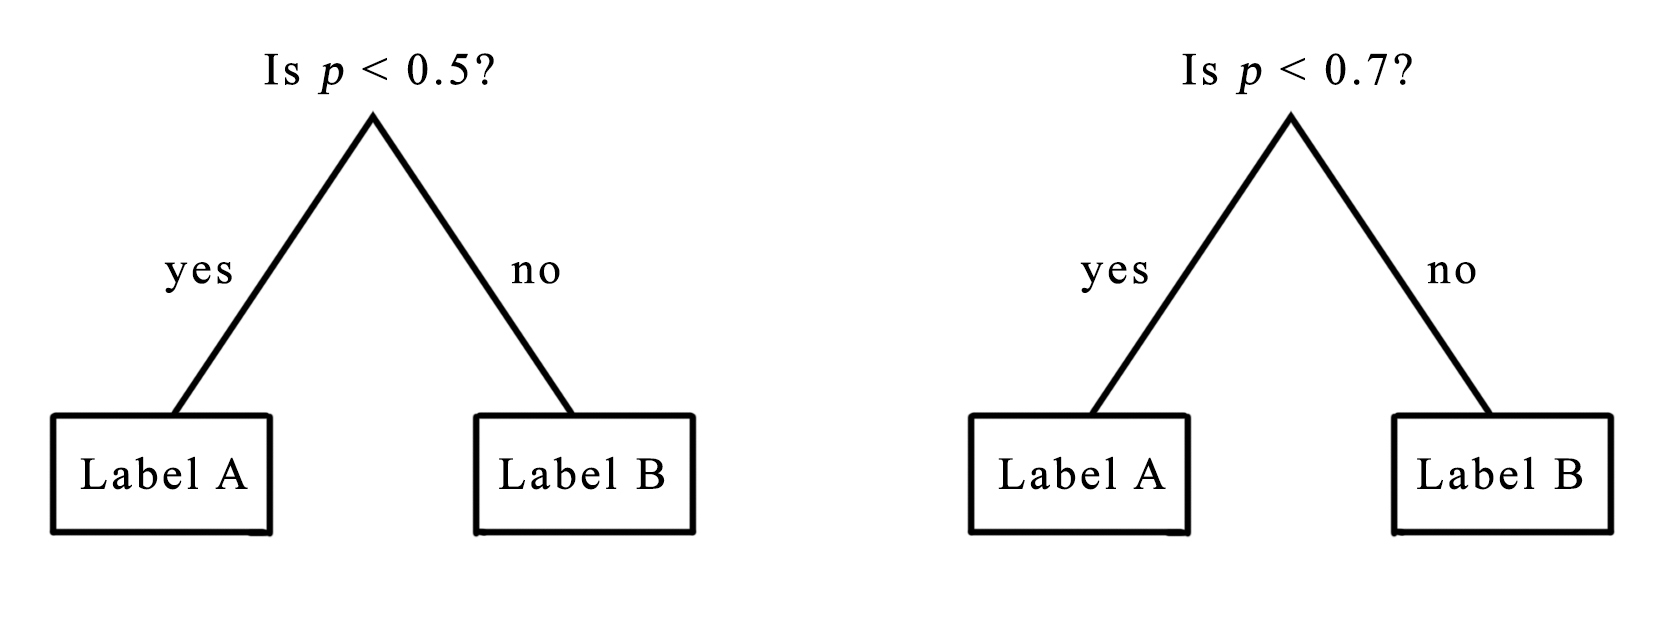
\includegraphics[width=0.75\linewidth]{ch-visualizer/figures/tree}
		\caption[Classifiers and classification models]{Although both figures 
		on the left and right are slightly different classifiers, they 
		are both instances of (extremely simple) decision trees.}
		\label{fig:visualizer:al:tree}
	\end{center}
\end{figure}

\subsection{Initialization of active learner}
\label{sec:visualizer:al:initialization}

It is problematic to start from scratch; how does the system determine
the best first point of ambiguity when it knows nothing (the hypothesis space is
everything)? A classic method is to simply select $k$ random data instances for 
the user to label. As initialization is not the focus of this work, the VS 
currently utilizes this methodology.

Alternatively, we can exploit the fact that the
user is already providing a numerical model that they believe to be a good
representation of the data which they would like the visualization system to
check visually. Given this data, the system builds a decision tree that utilizes
the various properties of the plots to determine whether one is interesting or
uninteresting. Doing so greatly narrows the hypothesis space and makes it easier
to determine points of ambiguity. However, to reconcile with the fact that the
user wishes to check the numerical model and may not necessarily believe it is a
good representation of fit, the learner must check whether the initial decision
tree is a proper fit (This may be achieved with line-up tests, which are 
described briefly in Section ~\ref{sec:futurework:lineup}). As the user then 
proceeds to label various conditional
plots as ``interesting'' or ``not interesting,'' the classifier learns the
user’s interest and continues to evolve. This models plot characteristics that
the user found interesting to study.

\subsection{Decision tree classification of user interests}
\label{sec:visualizer:al:tree}

Post-initialization, the active learner cleverly queries vital plots so that 
the system can best learn the user’s interests. The system first determines 
which features it is uncertain about classifying and then returns a plot 
matching those characteristics to the user. This allows the system to utilize 
its classification model of choice to build a better classifier more 
efficiently. It is important to distinguish between the active learner, which 
selects the next queries from the pool of unlabeled data, and the
classification model, which trains on labeled data to ``learn'' user interests 
and classify (predict) the remaining unlabeled data. 

A random forest is one model for classifying and labeling data (features of 
plots, in the case of the visualization system). In a random forest, various 
decision trees are constructed from random samples of the data. Each classifier 
has a vote of weight one for each unlabeled data, and the forest is aggregated 
by majority vote. It is easily presented to the 
analyst in the form of a decision tree, which aids in user 
interpretability of the system output. As such, the VS sets the choice of 
classification model to random forest by default.

\section{Automated plot generation (Stage 2)}
\label{sec:visualizer:plotgeneration}

\subsection{User interaction with active learning output}
\label{sec:visualizer:plotgeneration:user}

The system has now learned which of the unlabeled plots 
may be of interest to the user. The final learned classifier is used to fit the 
rest of the $d \choose 2$ unlabeled scatterplots, and a visual graph $G=(V,E)$ 
may be built from these labels with the following heuristic where $i,j \in 
\{1,...,d\}$:

\begin{algorithm}
	If label($i,j)>0$ (i.e. ``interesting'' instead of ``uninteresting''), draw 
	edge $E_{i,j}$
\end{algorithm}

Furthermore, the VS may provide a visualization of the resulting classifier 
itself such as the decision tree itself. The active learning output may be 
visualized as a heat map. A 
classic heat map represents each pair of variables as colors from a bivariate 
spectrum. Heat maps are difficult to interpret as it is one-dimensional; each 
end of the color spectrum represents minimum and maximum values respectively. 
It is unclear what the max or the min is as it depends on the domain of the 
whatever the heat map is plotting; as such, the minimum may not necessarily be 
negative while the maximum may not necessarily be positive. Furthermore, the 
subtle variations in hue between colors make it difficult to compare relative 
ranking among different pairs for colors that are similar. Buja \textit{et al.} 
propose an alternate, clearer method of visualizing the heat map, termed the 
``association navigator''~\cite{buja2016}. The association navigator is 
two-dimensional: the size of each color corresponds to its value while the 
color 
represents a positive or negative value~\cite{buja2016}. As such, the 
association navigator only utilizes two colors rather than a spectrum of 
colors, making it simple to distinguish between the two. By simplifying the 
color scheme and adding the dimension of size, the association navigator makes 
it much easier to interpret and compare different pairs of data at a glance. 
The stark difference between a traditional heatmap and the association 
navigator when applied to the same dataset may be seen in 
Figure~\ref{fig:visualizer:heatmap}. The VS provides both options, allowing the 
analyst to select whichever is easier to for them to interpret. 
With these visualizations of the active learning output, the user should be 
able to understand his/her own interests. 

\begin{figure}[htb]
	\begin{center}
		
\includegraphics[width=1\linewidth]{ch-visualizer/figures/vs}
		\caption[Heatmap versus association navigator]{Heatmap versus 
		association navigator example.}
		\label{fig:visualizer:heatmap}
	\end{center}
\end{figure}

\subsection{System output}
\label{sec:visualizer:plotgeneration:output}

There are three options at the end of stage 2. Two of them are concrete outputs 
that may be easily used in an analyst's final report, and the third is a 
refinement of the active learning component in stage 1.

\tablespacing
\begin{itemize}
	\item \textbf{Automatic plot generation:} The VS compiles a selection of 
	the most interesting and non-interesting plots along with their 
	associated transformation variables.
	\item \textbf{Graph comparison:} The VS accepts a numeric graph (For 
	example, a correlation graph $G^{\text{num}}$ generated with numerical 
	correlation 
	coefficients as described in Section~\ref{sec:intro:correlation}) and 
	measures the difference between the numeric graph $G^{\text{num}}$ and 
	visual graph $G$ (the active learning output). 
	Details on different graph comparison methods may be found in 
	Chapter~\ref{ch:gc}.
	\item \textbf{Lineup test:} In the event that the classifier is not a 
	satisfactory representation of the analyst's interests, the VS may utilize 
	lineup tests to help determine where to query from further. For more 
	details on this methodology, see Section~\ref{sec:futurework:lineup}.
\end{itemize}
\bodyspacing

With the focus on correlation graphs in this work, graph comparison is the most 
useful output from the visualization system. As such, it is one of our primary 
VS focuses. The next section provides a roadmap for the rest of this work, 
which goes into detail on two aspects of the VS. 
\section{Specific focus: AL and GC}
\label{sec:visualizer:focus}

The active learning component is the bread and butter of the visualization 
system and forms the first stage of the system. Furthermore, it solves for the 
tedious nature of classifying $d \choose 2$ plots in high-dimensional 
visualization , which was first brought up in Section~\ref{sec:intro:problem}. 
The second issue with high-dimensional visualization is the verification of the 
numerical results against the visual result. This is a question of the VS 
output, and graph comparison is a solution to this problem that is both 
informative to the analyst and further useful in the case of correlation 
graphs, which we are interested in for their financial applications. As such, 
the primary focus of this work that follows are active learning methods 
(Chapter~\ref{ch:al}) and graph comparison methods (Chapter~\ref{ch:gc}). These 
methods are applied to the current iteration of the VS, which is then utilized 
in conjugation with numerical correlation graphs to perform stock selection.

It should be noted that the VS is a large project and may certainly be further 
refined despite the work that we do to refine two major components of the 
system. Ideas for future extensions of the VS may be found in 
Section~\ref{sec:futurework}. There are several recommendations for 
improvements that can be made to different aspects of the system which are not 
the focus on this work.
